\documentclass[border=8pt]{standalone}
\usepackage{tikz,amsmath,amssymb,bm}
\usetikzlibrary{arrows.meta,calc,angles,quotes,decorations.markings}
\begin{document}
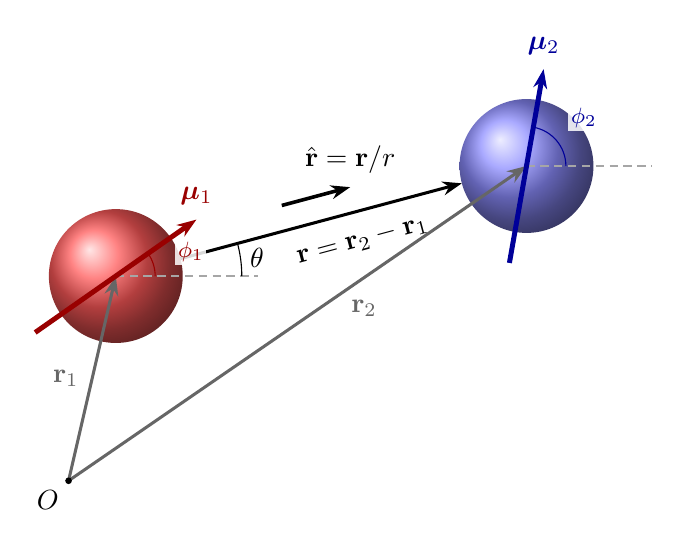
\begin{tikzpicture}[>={Stealth[length=7pt,width=5pt]},
  mom/.style={->,line width=1.8pt}, vec/.style={->,line width=1.1pt},
  aux/.style={densely dashed,gray!70},
  lbl/.style={fill=white,fill opacity=0.85,text opacity=1,inner sep=1pt,font=\footnotesize}]
\coordinate (O) at (-0.6,-2.6);
\coordinate (P1) at (0,0);\coordinate (P2) at (5.2160,1.3976);
\shade[ball color=red!65!white,opacity=1] (P1) circle (0.85);
\shade[ball color=blue!45!white,opacity=1] (P2) circle (0.85);

\draw[vec,gray!80!black] (O) -- (P1) node[midway,left=1pt] {$\mathbf r_1$};
\draw[vec,gray!80!black] (O) -- (P2) node[pos=0.6,below right=-1pt] {$\mathbf r_2$};
\fill (O) circle (1.2pt) node[below left] {$O$};
\draw[aux] (P1) -- ++(1.8,0) coordinate (X1);
\draw[aux] (P2) -- ++(1.6,0) coordinate (X2);
\draw[vec] ($(P1)!0.85 cm!(P2)$) -- ($(P2)!0.85 cm!(P1)$) node[pos=0.62,below=3pt,sloped] {$\mathbf r=\mathbf r_2-\mathbf r_1$};
\draw[vec,line width=1.3pt] ($(P1)!0.42!(P2)+(105:0.32)$) -- ++(15:0.9) node[above=1pt] {$\hat{\mathbf r}=\mathbf r/r$};
\draw[mom,red!60!black] (P1) ++(215:1.25) -- ++(35:2.5) node[above=1pt] {$\bm\mu_1$};
\draw[mom,blue!60!black] (P2) ++(260:1.25) -- ++(80:2.5) node[above=1pt] {$\bm\mu_2$};

\coordinate (T1) at (15:1.6);
\pic[draw,angle radius=1.6cm,"$\theta$",angle eccentricity=1.13] {angle=X1--P1--T1};
\coordinate (A1) at (35:1.0);
\pic[draw,red!60!black,angle radius=0.5cm,"$\phi_1$"lbl,angle eccentricity=2.0] {angle=X1--P1--A1};
\coordinate (A2) at ($(P2)+(80:1.0)$);
\pic[draw,blue!60!black,angle radius=0.5cm,"$\phi_2$"lbl,angle eccentricity=1.9] {angle=X2--P2--A2};
\end{tikzpicture}
\end{document}
